%-------------------------------------------------------------------------------
%                      Template Naskah Skripsi
%               	Berdasarkan format JTETI FT UGM
% 						(c) @gunturdputra 2014
%-------------------------------------------------------------------------------

%Template pembuatan naskah skripsi.
\documentclass{DTEDI_KP}

%Untuk prefiks pada daftar gambar dan tabel
\usepackage[titles]{tocloft}
\renewcommand\cftfigpresnum{Gambar\  }
\renewcommand\cfttabpresnum{Tabel\   }

%Untuk hyperlink dan table of content
\usepackage{hyperref}
\newlength{\mylenf}
\settowidth{\mylenf}{\cftfigpresnum}
\setlength{\cftfignumwidth}{\dimexpr\mylenf+2em}
\setlength{\cfttabnumwidth}{\dimexpr\mylenf+2em}

%Untuk Bold Face pada Keterangan Gambar
\usepackage[labelfont=bf]{caption}

%Untuk caption dan subcaption
\usepackage{caption}
\usepackage{subcaption}


%-----------------------------------------------------------------
%Disini awal masukan untuk data proposal skripsi
%-----------------------------------------------------------------
\titleind{RANCANG BANGUN KENDALI KINEMATIKA DAN ANTARMUKA ROBOT SCARA BERBASIS \emph{PROCESSSING}}

\fullname{IVAN SYAHRONI HERMAWAN}

\idnum{17/415746/SV/13611}

\approvaldate{4 Agustus 2019}

\degree{Diploma Teknologi Listrik}

\yearsubmit{2019}

\program{Teknologi Listrik}

\dept{Departemen Teknik Elektro dan Informatika}

\firstsupervisor{Ma'un Budiyanto, S.T., M.T.}
\firstnip{197007071999031002}

\secondsupervisor{Fahmizal, S.T., M.Sc}
\secondnip{111198807201609101}

%-----------------------------------------------------------------
%Disini akhir masukan untuk data proposal skripsi
%-----------------------------------------------------------------

\begin{document}

\cover

\approvalpage

%-----------------------------------------------------------------
%Disini awal masukan Acknowledment
%-----------------------------------------------------------------


%-----------------------------------------------------------------
%Disini awal masukan untuk Prakata
%-----------------------------------------------------------------
\preface
Assalamu'alaikum Wr. Wb.

\vspace{0.5cm}

Puji syukur penulis panjatkan ke hadirat Allah SWT karena hanya dengan rahmat dan hidayah-Nya, Kerja Praktik ini dapat terselesaikan tanpa halangan berarti. Keberhasilan dalam menyusun laporan Kerja Praktik ini tidak lepas dari bantuan berbagai pihak yang mana dengan tulus dan ikhlas memberikan masukan guna sempurnanya Kerja Praktik ini. Oleh karena itu dalam kesempatan ini, dengan kerendahan hati penulis mengucapkan terima kasih kepada:

\begin{enumerate}
\item{Bapak 	Ma'un Budiyanto, S.T., M.T. selaku Ketua  Program Studi Teknologi Listrik Universitas Gadjah Mada,}
\item{Bapak Fahmizal, S.T., M.Sc selaku dosen pembimbing pertama yang telah memberikan banyak bantuan, bimbingan, serta arahan dalam Kerja Praktik,}
\item{Seluruh Dosen di Teknologi Listrik Sekolah Vokasi Universitas Gadjah Mada, yang tidak bisa disebutkan satu-satu, atas ilmu dan bimbingannya,}
\item{Ibu dan Bapak yang selama ini telah sabar membimbing, mengarahkan, dan mendoakan penulis tanpa kenal lelah untuk selama-lamanya, dan}

\end{enumerate}

Penulis menyadari bahwa penyusunan Kerja Praktik ini jauh dari sempurna. Kritik dan saran dapat ditujukan langsung pada \emph{e-mail} saya. Akhir kata penulis mohon maaf yang sebesar-besarnya apabila terdapat kekeliruan di dalam penulisan Kerja Praktik ini.

\vspace{0.5cm}

Wassalamu'alaikum Wr. Wb.

\begin{tabular}{p{7.5cm}c}
&Yogyakarta, 5 Agustus 2019\\
&\\
&\\
&\textbf{Penulis}
\end{tabular}

%-----------------------------------------------------------------
%Disini akhir masukan untuk muka skripsi
%-----------------------------------------------------------------
\tableofcontents
\addcontentsline{toc}{chapter}{DAFTAR ISI}
\listoftables
\addcontentsline{toc}{chapter}{DAFTAR TABEL}
\listoffigures
\addcontentsline{toc}{chapter}{DAFTAR GAMBAR}

%-----------------------------------------------------------------
%Daftar Singkatan [Optional]
%-----------------------------------------------------------------

%-----------------------------------------------------------------
%Disini awal masukan Intisari
%-----------------------------------------------------------------
\begin{abstractind}
	Penelitian ini bertujuan untuk melakukan pengoperasian terhadap robot SCARA. SCARA merupakan akronim untuk \emph{Selective Compliance Assembly Robot Arm} dimana robot ini dapat bergerak dalam dua aksis, yaitu horisontal dan vertikal. Pergerakan Robot ini menggunakan kedua lengan untuk pergerakan horisontal dan satu lengan untuk pererakan vertikal. Robot SCARA ini dioperasikan dengan bantuan antar muka yang dibuat dari \emph{Processing} yang dibuat menggunakan program bahasa c. Antarmuka yang ditampilkan menunjukan pengoperasian robot SCARA mulai dari kinematika maju dan kinematika balik.


\bigskip
\noindent
\textbf{Kata kunci :} SCARA, \emph{Processing}, Kendali, \emph{inverse kinematic, Forward Kinematics}.
\end{abstractind}
	
\begin{abstracteng}
\emph{
This study aims to carry out operations on the SCARA robot. SCARA is an acronym for \ emph {Selective Compliance Assembly Robot Arm} where this robot can move in two axes, namely horizontal and vertical. Movement This robot uses both arms for horizontal movement and one arm for vertical movement. This SCARA robot is operated with the help of an interface created from \ emph {Processing} made using a language program c. The interface shown shows the operation of the SCARA robot from forward kinematics and back kinematics.}


\bigskip
\noindent
\textbf{\emph{Keywords :}} \emph{SCARA, \emph{Processing}, Control.}.
\end{abstracteng}
%-----------------------------------------------------------------
%Disini akhir masukan Intisari
%-----------------------------------------------------------------

%-----------------------------------------------------------------
%Disini awal masukan untuk Bab
%-----------------------------------------------------------------
%!TEX root = ./template-skripsi.tex
%-------------------------------------------------------------------------------
% 								BAB I
% 							LATAR BELAKANG
%-------------------------------------------------------------------------------

\chapter{LATAR BELAKANG}

\section{Latar Belakang Masalah}
	Robotika merupakan salah satu bidang ilmu yang mempelajari desain, modeling, dan kendali robot. Saat ini, robot memiliki peranan yang penting dalam membantu pekerjaan manusia, contohnya dalam bidang industri. Dalam bidang industri, robot umumnya terdapat pada proses manufaktur seperti proses pengelasan, \textit{spray painting}, perakitan, \textit{milling} dan \textit{drilling} dapat dikerjakan dengan sebuah robot secara terus menerus dan berulang secara otomatis. Salah satu robot dalam proses manufaktur adalah Robot SCARA. Robot SCARA atau \emph{Selective Compilance Assembly Robot Arm} dalam dunia industri umumnya digigunakan dalam pemilahan barang. 
	
Robot SCARA dapat bergerak secara optimal dan efisien karena sebuah persamaan kinematika. Persamaan kinematika yang diguanakan adalah \textit{inverse kinematic} dengan input berupa titik koordinat kartesius \textit{($x_{1}$,$y_{2}$)} dan output berupa nilai sudut untuk mengendalikan motor servo pada \textit{shoulder} dan \textit{elbow}.

Dalam membangun sebuah sistem kendali, dibutuhkan \textit{platfrom} antar muka sebagai jembatan antara \textit{user} dengan \textit{hardware}. Dalam penelitian ini program antar muka dirancang menggunakan \textit{software} Processing Ide. \emph Software ini memiliki beberapa keunggulan yang membuatnya lebih efektif dan cukup mudah untuk digunakan sebagai \textit{platform} antar muka. Keunggulan tersebut salah satunya ialah mudahnya sarana komunikasi terhadap \emph hardware yang digunakan. \emph Processing Ide juga dapat melakukan komunkasi dua arah yang berarti antara antar muka dan juga \emph hardware yang digunakan dapat saling berkirim data dan juga menerima data.
Oleh Karena itu, pada program kerja praktik ini dilakukan analisis robot SCARA berupa kinematika maju dan kinematika balik dengan perancangan antar muka berbasis \emph Processing Ide. Atas dasar tersebut penulis membuat judul kerja praktik berjudul "\textbf{Rancang Bangun Kendali Kinematika dan Antar Muka Robot SCARA Berbasis Processing Ide}" guna memberikan inovasi dan pengembangan pada sistem kendali kinematika pada robot SCARA yang dapat diimplementasikan sebagai sarana belajar sistem kendali di Laboratorium Instrumentasi dan Kendali Sekolah Vokasi Universitas Gadjah Mada.\\

\section{Tujuan}
Tujuan penulis melakukan penelitian dibagi menjadi dua, yaitu tujuan secara umum dan tujuan secara khusus.

\subsection{Tujuan Umum}

Memenuhi salah satu syarat kelulusan program kerja praktik program studi Teknologi Listrik Sekolah Vokasi Universitas Gadjah Mada.

\subsection{Tujuan Khusus}

\begin{enumerate}
	\item Merancang sistem kinematika robot SCARA, baik kinematika maju maupun balik,
	\item Merancang antarmuka penggunaan robot SCARA dengan \emph {software Processing Ide.}
\end{enumerate}


\section{Metode Kerja Praktik}
Pengerjaan dan penyusunan Kerja Praktik ini menggunakan beberapa metode.

\begin{enumerate}
	\item Metode pustaka\\
	Metode dengan memahami dan mempelajari berbagai jurnal yang berkaitan dengan robot SCARA, gerak kinematika, dan \emph {Processing Ide}.
	\item Metode perancangan alat\\
	Metode dengan melakukan pembuatan desain elektronis dan mekanis, pemrograman, serta perancangan antarmuka menggunakan \emph{ Processing Ide].
	\item Metode pengujian\\
	Metode dengan melakukan pengujian terhadap paramater-parameter yang dibutuhkan seperti pergerakan dari motor servo, pembacaan nilai umpan balik dari motor oleh potensiometer, serta pengujian terhadap kinematika robot SCARA yang tertampil pada antarmuka \emph {Processing Ide.}

\end{enumerate}

\section{Sistematika Penulisan}
Penulisan laporan Kerja praktik ini dilakukan dengan mengikuti sistematika sebagai berikut:\\
\noindent
\textbf{BAB I\hspace*{0.6cm}: PENDAHULUAN}\\
\noindent
Memuat latar belakang masalah, maksud dan tujuan, batasan masalah, metodologi penetilian, dan sistematika penulisan.\\
\noindent
\textbf{BAB II\hspace*{0.5cm}: LANDASAN TEORI}\\
\noindent
Memuat gambaran umum robot SCARA, kinematika maju dan kinematika balik, dan \emph{Processing Ide.}\\
\textbf{BAB III\hspace*{0.375cm}:  PERANCANGAN SISTEM}\\
\noindent
Memuat perancangan sistem secara umum, dimulai dari perancangan elektronis, mekanis, pemrograman hingga pada antarmuka \emph {processing ide.}\\
\textbf{BAB IV\hspace*{0.4cm}: PENGUJIAN SISTEM}\\
\noindent
Memuat pengujian dan anilisa terhadap hasil yang didapat seperti analisa kerja dari sistem penggerak, pembacaan sensor, serta pengujian sistem secara keseluruhan dengan \emph {processing ide.}
\\
\textbf{BAB V\hspace*{0.6cm}: PENUTUP}
Memuat kesimpulan dari perancangan hingga pada hasil pengujian, dan berisi saran-saran untuk pengembangan lebih lanjut.
\\



% Baris ini digunakan untuk membantu dalam melakukan sitasi
% Karena diapit dengan comment, maka baris ini akan diabaikan
% oleh compiler LaTeX.
\begin{comment}
\bibliography{daftar-pustaka}
\end{comment}


%!TEX root = ./template-skripsi.tex
%-------------------------------------------------------------------------------
%                            BAB II
%               TINJAUAN PUSTAKA DAN DASAR TEORI
%-------------------------------------------------------------------------------

\chapter{TINJAUAN PUSTAKA DAN DASAR TEORI}                


\section{Landasan Teori}

  \subsection{SCARA}
  \begin{figure}[H]
  	\centering
  	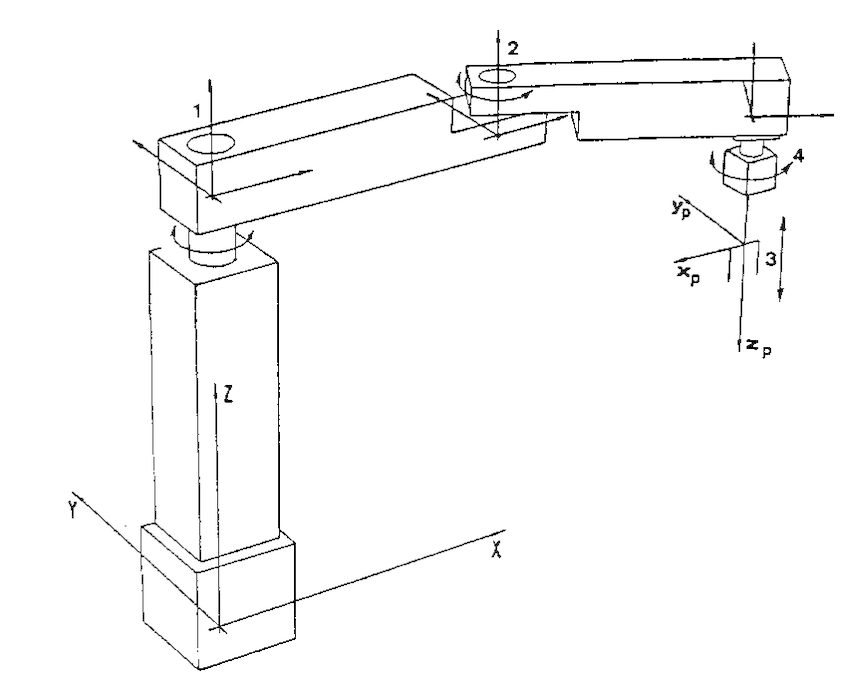
\includegraphics[width=4.33cm]{scara.png}
  	\caption{Pergerakan Robot SCARA}
  \end{figure}
  
  SCARA merupakan singkatan dari \emph{Selective Compliant Assembly Robot Arm}. Robot ini pertama kali dibuat oleh perusahaan USA bernama Adept pada 1984 dan diklasifikasikan sebagai robot industri. Sistem penggerak robot SCARA merupakan pergerakan langsung pada lengan tanpa bantuan sistem \emph{belt} keculai pada bagian \emph wirst, sehingga membuat mekanisme gerakannya bekerja cepat, sederhana namun tetap akurat. Robot ini banyak digunakan sebagai robot \emph {aseembly part} dengan ukuran yang kecil degan kecepatan sedang. 
  
  Robot SCARA yang digunakan pada penelitian ini menggunakan robot SCARA dengan nama Serpent-2. Robot Serpent-2 memiliki dua \textit{horizontal joint} yaitu bagian \textit{shoulder, elbow}dan \textit{wrist} yang dikendalikan oleh motor servo. Sedangkan pada bagian \textit{vertical joint} yang berfungsi sebagai naik turun dan buka tutup dari \emph wirst, dikendalikan oleh pneumatik yang dikontrol oleh \emph {valve relay}. Sehingga, gerakan yang terdapat pada robot SCARA dapat diklasifikasikan sebagai gerakan mengambil dan menempatkan objek. 
  \begin{table}[H]
  	\centering
  	\caption{Spesifikasi Robot Serpent-2}
  	\resizebox{6cm}{!}{%
  		\begin{tabular}{|l|l|}
  			\hline
  			Main arm length      & 360 mm$$\hspace{2cm} 		\\ \hline
  			Fore arm length      & 290 mm$$  				\\ \hline
  			Shoulder movement    & 180 °$$  		\\ \hline
  			Elbow movement       & 200 °$$   		\\ \hline
  			Wrist rotation       & 360 °$$ 		\\ \hline
  			Up \& down movement  & 150 mm$$   				\\ \hline
  			Maximum tip velocity & 3.0 kg$$  				\\ \hline

  		\end{tabular}%
  	}
  \end{table}

 Pada bagian motor servo, robot serpent-2 menggunakan tiga buah sensor \emph feedback yang berguna sebagai pemberi nilai posisi pada masing-masing motor servo. Sensor \emph feedback yang digunakan pada robot SCARA ini menggunakan potensiometer yang memberikan nilai analog dan kemudian diproses oleh Arduino Mega 2560. Nilai ini, nantinya untuk memproses gerak kinematika dari robot SCARA tersebut sesuai dengan posisi yang diinginkan.
 \begin{table}[H]
 	\centering
 \caption{Spesifikasi Motor DC pada robot Serpent-2}
 \resizebox{11cm}{!}{%
 	\begin{tabular}{|l|l|}
 		\hline
 		Moments of inertia of the main arm ($J_{1}$)    							& $$ 				\\ \hline
 		Moments of inertia of the fore arm ($J_{2}$)    							& $$ 				\\ \hline
 		Masses of the main arm	($m_{1}$)											& $$   					\\ \hline
 		Masses of the fore arm  ($m_{2}$)     										& $$   					\\ \hline
 		Motor and equivalent inertias ($J_{m}$)      								& $$ 			\\ \hline
 		Back emf constants for main arm and fore arm motor ($K_{e1}=K_{e2}$)  		& $$   				\\ \hline
 		Armature resistance for main arm and fore arm motor($R_{a1}=R_{a2}$)		& $$  					\\ \hline
 		Armatures inductances for main and fore arm motor  ($L_{a1}=L_{a2}$) 		& $$ 						\\ \hline
 	\end{tabular}%
 }
\end{table}


  \subsection{Kinematika Robot}
  Kinematika robot adalah studi analisis
  pergerakan kaki atau lengan robot terhadap
  sistem kerangka koordinat acuan yang diam
  atau bergerak tanpa memperhatikan gaya yang
  menyebabkan pergerakan tersebut. Model
  kinematika merepresentasikan hubungan \emph{end
  effector} dalam ruang tiga dimensi dengan
  variabel sendi dalam ruang sendi.
  
  Dalam kinematika dikenal istilah \emph{forward}
  kinematika dan \emph{invers} kinematika. \emph{Forward}
  kinematika adalah metode untuk menentukan
  orientasi dan posisi \emph{end effector} dari besarnya
  sudut sendi dan panjang link kaki robot.
  Sedangkan \emph{invers} kinematika merupakan
  kebalikan dari forward kinematika yaitu metode
  untuk mengetahui nilai sudut pada sendi-sendi
  yang diperlukan agar end effector dapat
  mencapai posisi yang dikehendaki. 
  
   \subsection{Arduino Mega 2560}
   \begin{figure}[H]
   	\centering
   	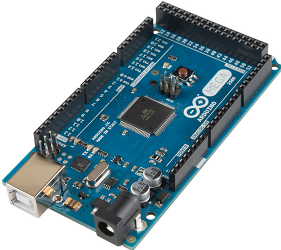
\includegraphics[width=4.33cm]{gambar/arduino_mega.png}
   	\caption{ Arduino Mega 2560}
   \end{figure}
   
  Board Arduino Mega 2560 adalah sebuah Board Arduino yang menggunakan IC Mikrokontroler ATmega 2560.Board ini memiliki Pin I/O yang relatif banyak, 54 digital Input / Output,15 buah di antaranya dapat digunakan sebagai output PWM, 16 buah analog Input, 4 UART. Arduino Mega 2560 di lengkapi cristal 16. Mhz 
  	
  
   \subsection{Processing IDE}
  \begin{figure}[H]
  	\centering
  	
\includegraphics[width=4.33cm]{logo_processing.png}
  	\caption{Processing IDE}
  \end{figure}
  \emph{Processing} adalah lingkungan pemrograman sederhana yang dibuat untuk  memudahkan pengembangkan aplikasi yang berorientasi visual dengan penekanan pada animasi dan menyediakan respon balik yang instan kepada pengguna melalui interaksi didalamnnya. Para pengembang menginginkan cara untuk "membuat sketsa" ide dalam kode. Karena kemampuannya telah berkembang selama dekade terakhir, \emph{Processing} telah digunakan untuk pekerjaan tingkat produksi yang lebih maju. Awalnya dibangun sebagai ekstensi khusus domain ke Java yang ditargetkan untuk seniman dan desainer, Processing telah berevolusi menjadi desain penuh dan alat \emph{prototyping} yang digunakan untuk pekerjaan instalasi skala besar, gambar gerak, dan visualisasi data yang kompleks.
   

  
  

% Baris ini digunakan untuk membantu dalam melakukan sitasi
% Karena diapit dengan comment, maka baris ini akan diabaikan
% oleh compiler LaTeX.
\begin{comment}
\bibliography{daftar-pustaka}
\end{comment}


%!TEX root = ./template-skripsi.tex
%-------------------------------------------------------------------------------
%                            BAB III
%               		METODOLOGI PENELITIAN
%-------------------------------------------------------------------------------

\chapter{PERANCANGAN SISTEM}

\section{Metode Perancangan sistem}
Perancangan robot serpent-2 ini diawali dengan menentukan metode yang tepat untuk mendesain dan membangun sistem secara keseluruhan meliputi perancangan elektronis,pemrograman pada Arduino Mega 2560, implementasi kinematika robot pada robot serpent-2, serta perancangan antarmuka pada \emph {processing ide}.Metode perancangan sistem meliputi diagram blok, flowchart cara kerja sistem, prinsip kerja dan perancangan tiap segmen-segmen yang dibutuhkan.
\subsection{Diagram Blok Perancangan Sistem}
Pada dasarnya, perancangan sistem untuk robot serphent-2 secara sederhana dapat dibagi menjadi tiga bagian. Ketiga perancangan ini merupakan hal yang sangat penting dan saling berkaitan.Perancangan robot serphent=2 jika digambarkan dalam diagram blok sistem dapat digambarkan seperti yang ditunjukkan dalam gambar 3.1
	\begin{figure}[H]
	\centering
	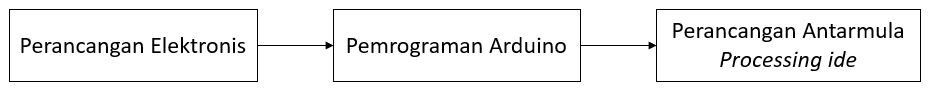
\includegraphics[width=\linewidth]{001.jpg}
	\caption{Diagram metode perancangan sistem.}
\end{figure}
	
\subsection{Flowchart Cara Kerja Sistem}
Kerja sistem, merupakan bagaimana robot serphent-2 melakukan tugasnya sesuai perintah yang dimasukkan dan kemudian dilaksanakan oleh aktuator.Robot serphent-2 memiliki kerja sistem yang tergolong ringkas yang mana didominasi oleh sistem maju tetapi juga memiliki sistem balik.  Kerja sistem dari robor serphent 2 jika dirancang dalam bentuk flowchat dapat ditunjukkan seperti dalam gambar 3.2

	\begin{figure}[H]
	\centering
	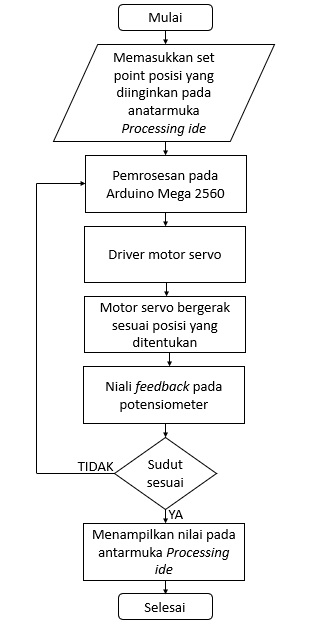
\includegraphics[width=8cm	]{002.png}
	\caption{Flowchat cara kerja sistem.}
\end{figure}

\subsection{Perancangan Elektronis}
Perancangan elektronis merupakan perancangan dasar pada pembuatan suatu sistem. Suatu sistem dapat bekerja secara maksimal karena terdiri dari komponen-komponen yang memiliki fungsi masing-masing. Komponen-komponen ini, disatukan kedalam sebuah \textit{Shield} \textit{Printed Circuit Board} (PCB). 

	\begin{enumerate}
\item Pengendali motor DC yang digunakan adalah modul EMS 30A H-Bridge sebanyak tiga buah yang masing-masing untuk menggerakkan \textit{Shoulder, Elbow} dan perputaran \textit{Wrist}. Secara garis besar, fungsi modul pengendali motor ini adalah untuk mengendalikan arah dan kecepatan putaran motor DC sesuai instruksi kendali dari Arduino Mega 2560 pengguna.Modul akan menerima nilai yanf dikirimkan oleh Arduino Mega 2560 dan kemudian menggerakan motor servo yang sudah terhubung dengan \textit{shoulder, Elbow} dan perputaran dari \textit{Wirst}.

\begin{figure}[H]
	\centering
	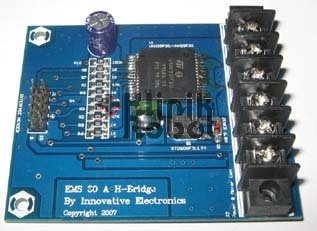
\includegraphics[width=5cm	]{driver_motor.jpg}
	\caption{Pengendali Motor DC EMS 30A H-Bridge}
\end{figure}

\item Potensiometer yang digunakan adalah jenis potensiometer \textit{rotary}. Potensiometer ini sebagai sensor posisi motor servo. Potensiometer terpasang pada setiap bagian motor servo sesuai dengan perputarannya dan akan memberikan keluaran berupa level tegangan yang berubah-ubah sesuai dengan posisi motor servo saat itu. Level tegangan tersebut kemudian dikirimkan kepada Arduino Mega 2560 sebagai sensor \textit{feedback} yang nantinya akan diproses untuk menyempurnakan posisi sesuai yang ditentukan.
\begin{figure}[H]
	\centering
	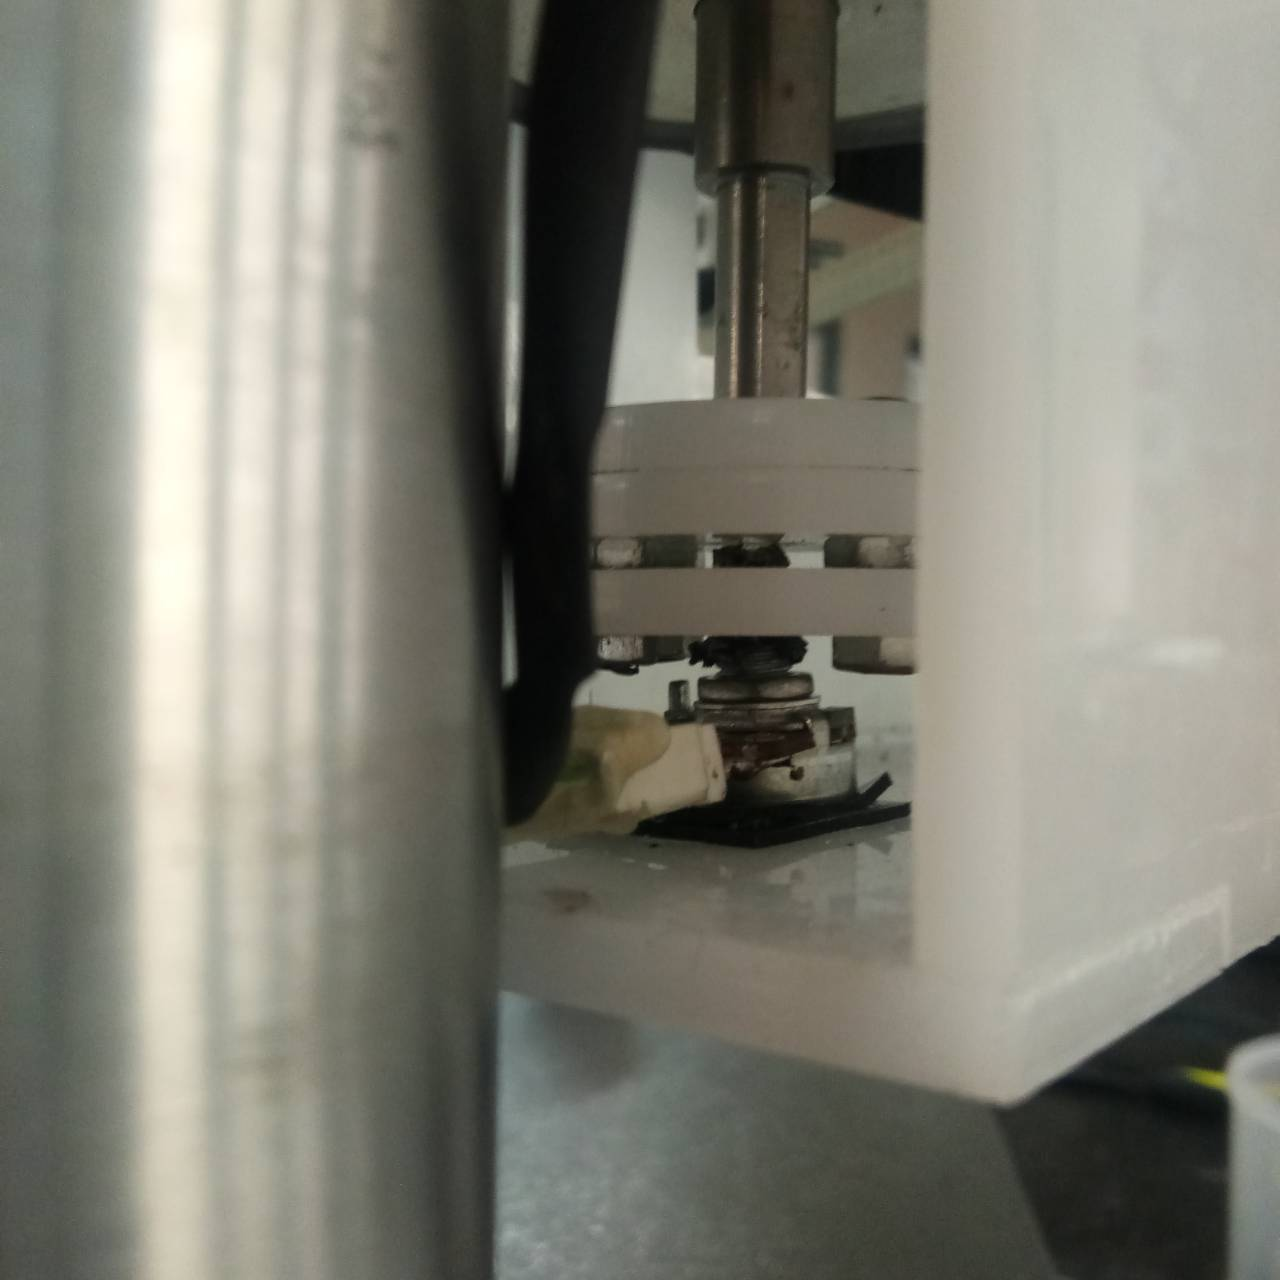
\includegraphics[width=5cm	]{potensio.jpg}
	\caption{Mekanisme pemasangan potensiometer pada motor}
\end{figure}

\item Pengaturan pergerakan vertikal dari \textit{wirst} pada robot serphent-2 menggunakan sistem pneumatik silinder. Pada bagian buka tutup \textit{wirst} menggunakan masukan udara biasa untuk menutupnya dan membuang udara unutk membukanya. Udara tersebut didapat dari kompresor yang terhubung melalui selang dan dikontrol melalui sebuah relay yang bekerja pada tegangan 24v.

\begin{figure}[H]
	\centering
	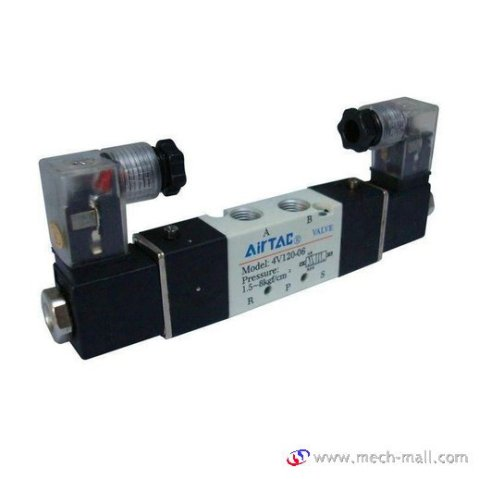
\includegraphics[width=5cm	]{relay.jpg}
	\caption{Relay pneumatik}
\end{figure}
\begin{figure}[H]
	\centering
	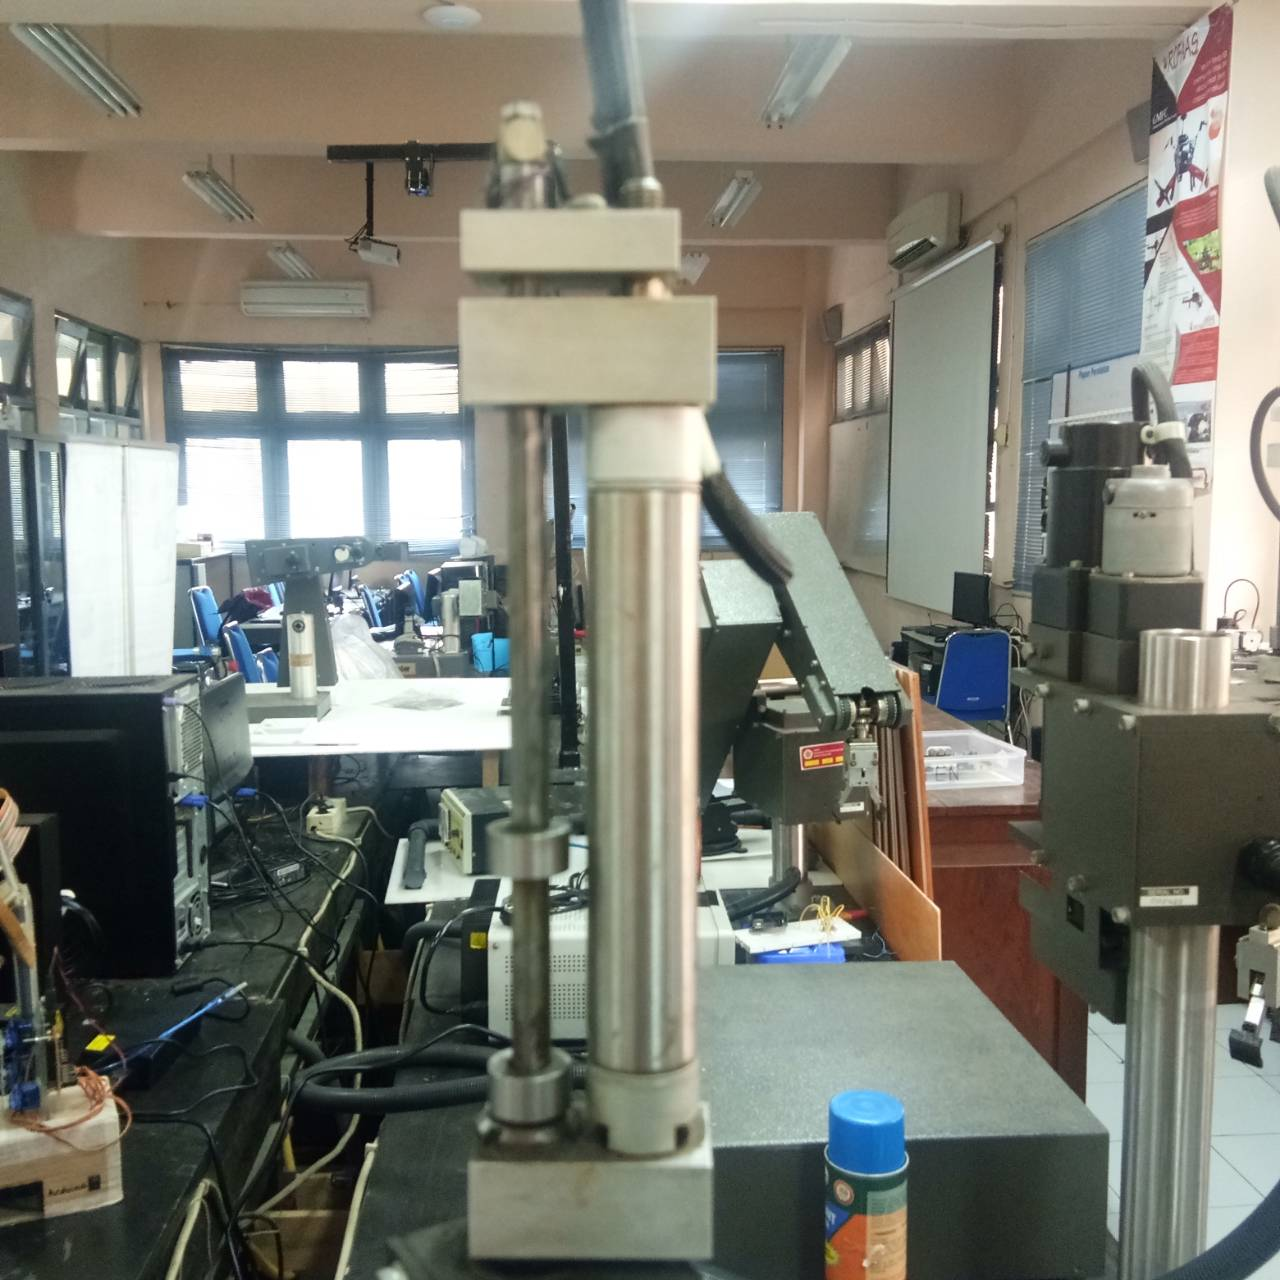
\includegraphics[width=5cm	]{relay2.jpg}
	\caption{Pneumatik Silinder}
\end{figure}

\item Relay yang bekerja pada tegangan 24v, pada Arduino Mega 2560 dikontrol melalui sinyal digital dengan bantuan rangkaian yang menggunakan TIP31A yang berfungsi untuk memutus atau membuka tegangan 24v. 
\begin{figure}[H]
	\centering
	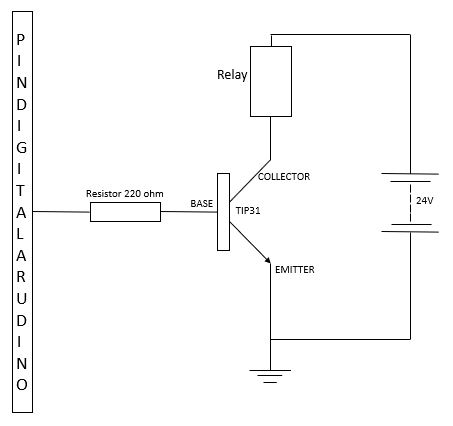
\includegraphics[width=5cm	]{relay3.jpg}
	\caption{Rangkaian skematik TIP31 sebagai \textit{switch}}
\end{figure}

\item Semua komponen-komponen yang dibutuhkan pada sistem kerja, disatukan ke dalam \textit{shield PCB} yang bertujuan agar meringkaskan serta memudahkan perangkaian elektronis. Rangkaian PCB dibuat melalui \textit{software} Eagle.
\begin{figure}[H]
	\centering
	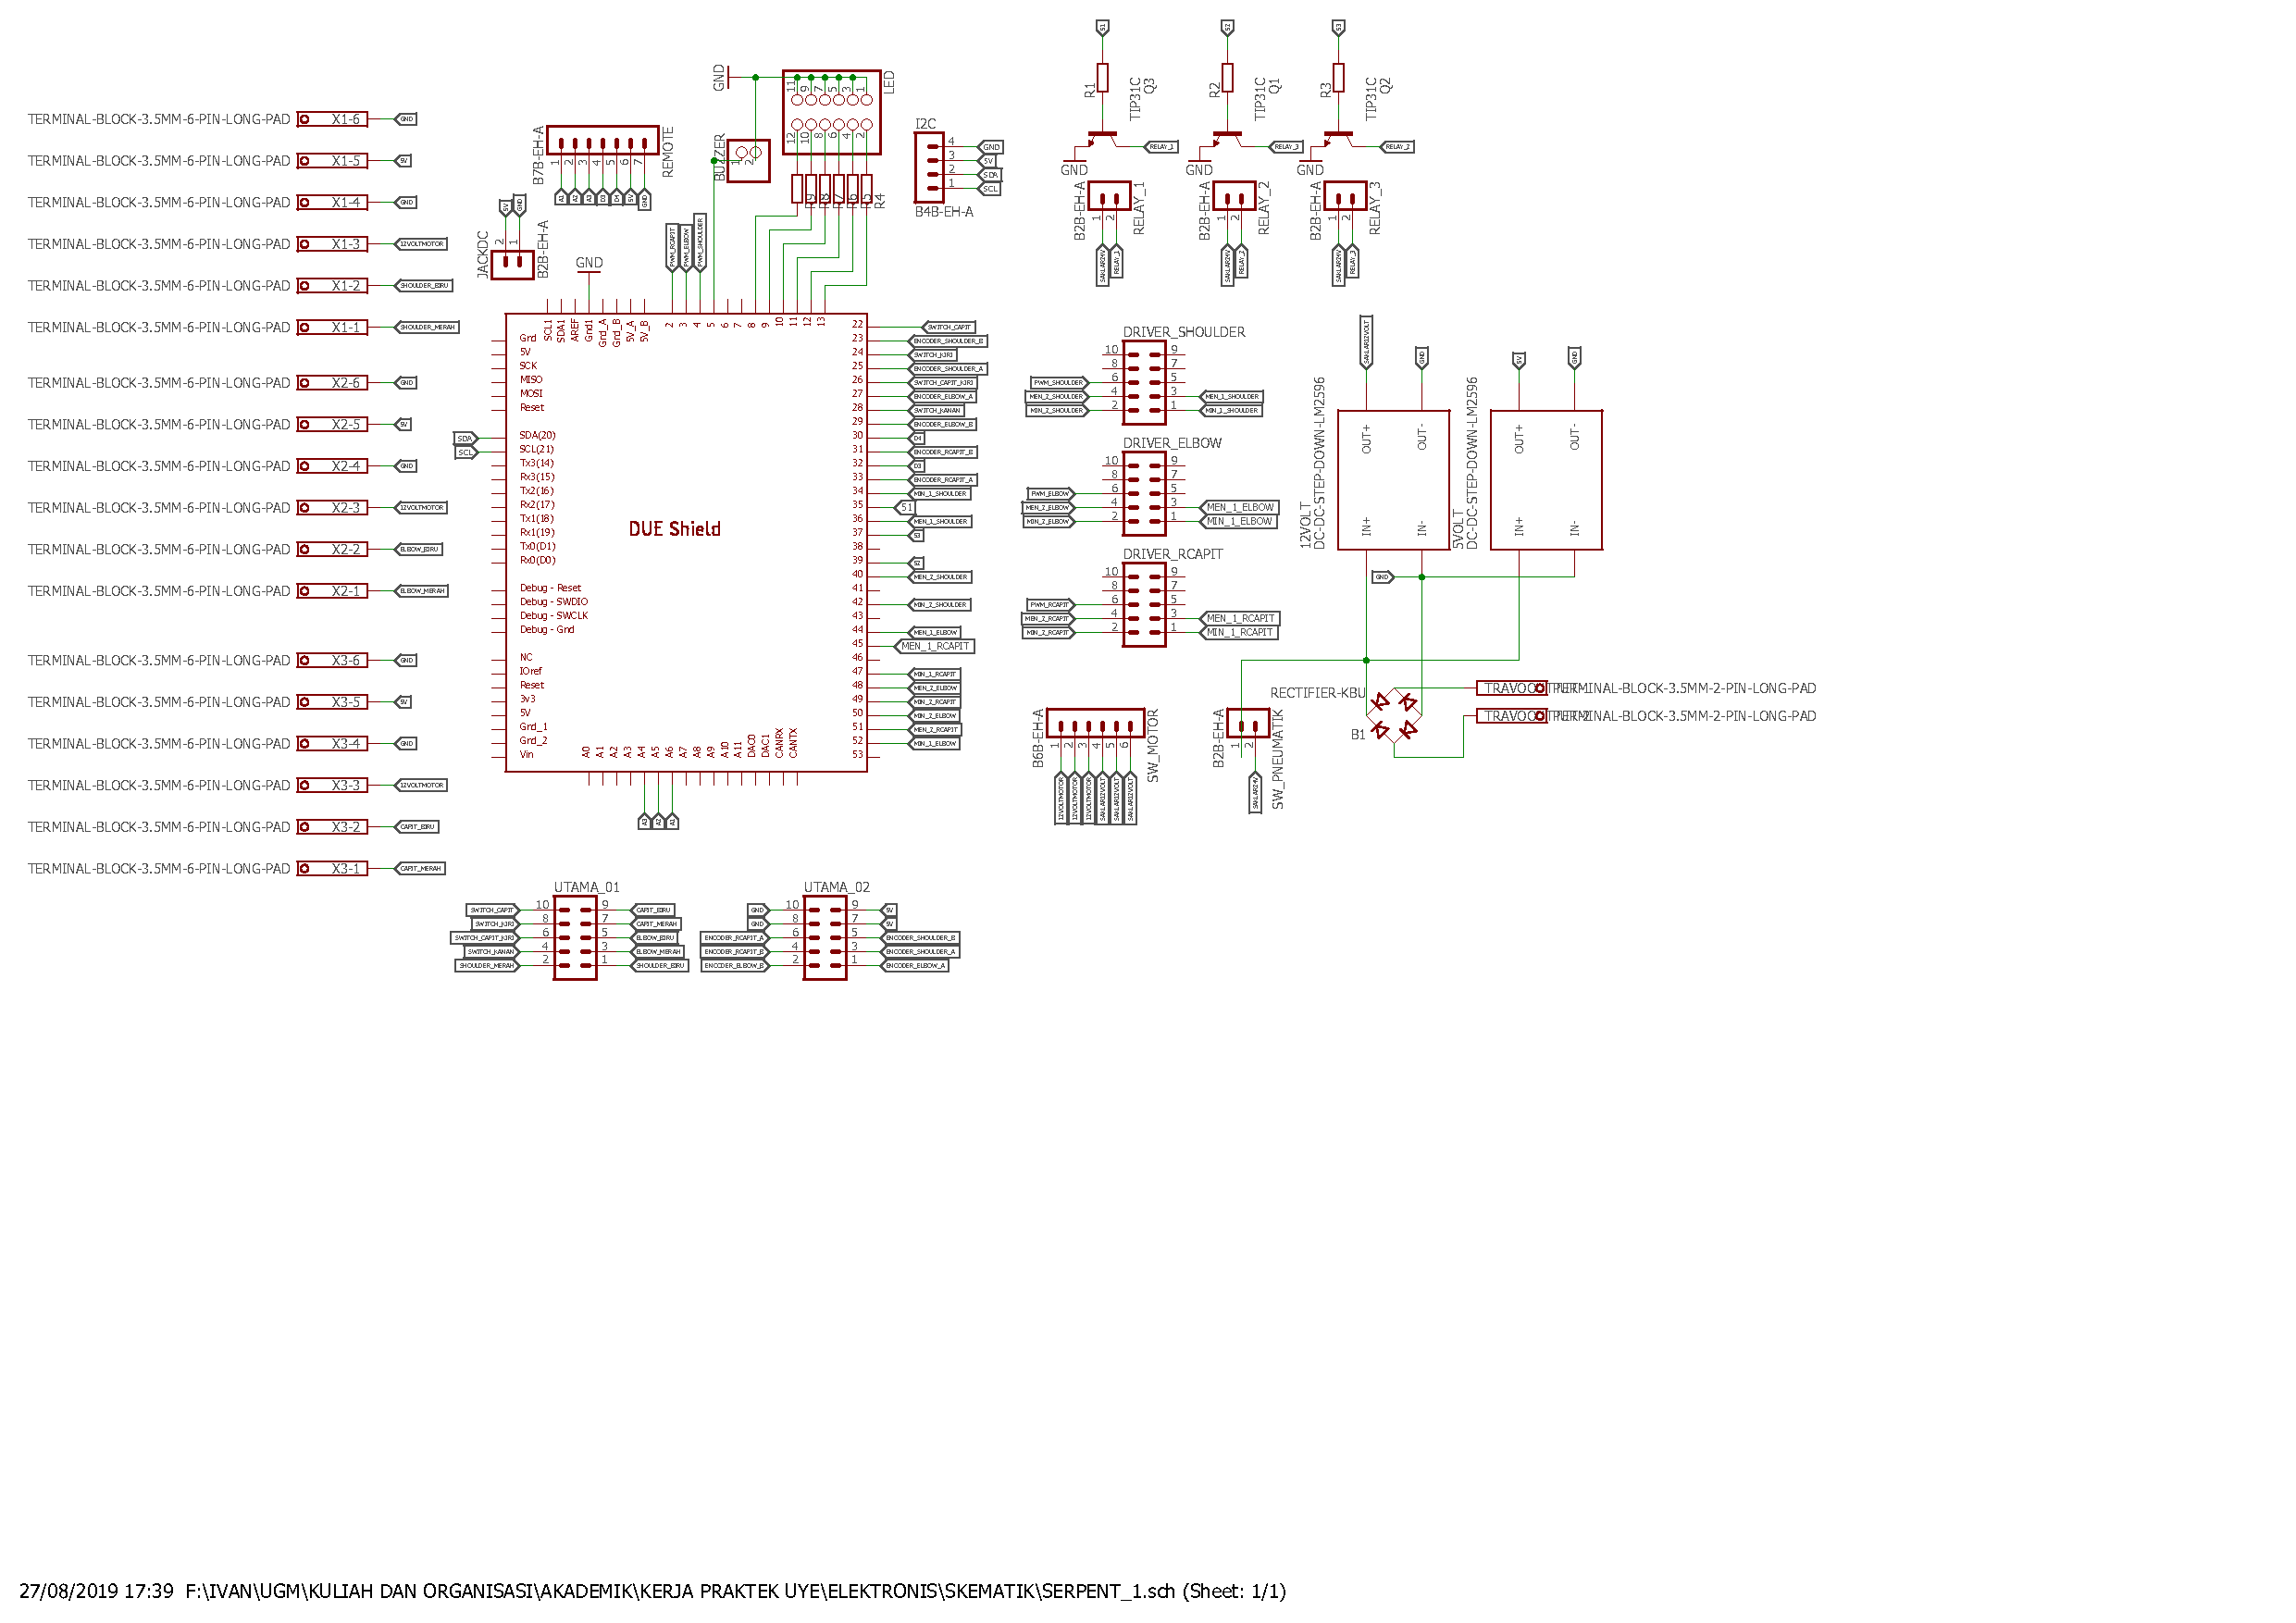
\includegraphics[width=15cm	]{skematik.pdf}
	\caption{Skematik rangkaian elektronis keseluruhan}
\end{figure}


		\end{enumerate}
	
\subsection{Perograman Arduino}
\subsection{Peranacangan Antarmuka \textit{Processing ide}}
	
% Baris ini digunakan untuk membantu dalam melakukan sitasi
% Karena diapit dengan comment, maka baris ini akan diabaikan
% oleh compiler LaTeX.
\begin{comment}
\bibliography{daftar-pustaka}
\end{comment}


%!TEX root = ./template-skripsi.tex
%-------------------------------------------------------------------------------
%                            BAB IV
%               		HASIL DAN PEMBAHASAN
%-------------------------------------------------------------------------------

\chapter{PENGUJIAN SISTEM}
% Baris ini digunakan untuk membantu dalam melakukan sitasi.
% Karena diapit dengan comment, maka baris ini akan diabaikan
% oleh compiler LaTeX.
\begin{comment}
\bibliography{daftar-pustaka}
\end{comment}

%!TEX root = ./template-skripsi.tex
%-------------------------------------------------------------------------------
%                            	BAB V
%               		KESIMPULAN DAN SARAN
%-------------------------------------------------------------------------------

\chapter{KESIMPULAN DAN SARAN}

\section{Kesimpulan}
	Berdasarkan hasil analisis dan pengujian fungsional aplikasi ini, didapat kesimpulan sebagai berikut:



\section{Saran}

	

	
% Baris ini digunakan untuk membantu dalam melakukan sitasi
% Karena diapit dengan comment, maka baris ini akan diabaikan
% oleh compiler LaTeX.
\begin{comment}
\bibliography{daftar-pustaka}
\end{comment}


%-----------------------------------------------------------------
%Disini akhir masukan Bab
%-----------------------------------------------------------------


%-----------------------------------------------------------------
% Disini awal masukan untuk Daftar Pustaka
% - Daftar pustaka diambil dari file .bib yang ada pada folder ini
%   juga.
% - Untuk memudahkan dalam memanajemen dan menggenerate file .bib
%   gunakan reference manager seperti Mendeley, Zotero, EndNote,
%   dll.
%-----------------------------------------------------------------
\bibliography{IEEEabrv,daftar-pustaka}
\addcontentsline{toc}{chapter}{DAFTAR PUSTAKA}
%-----------------------------------------------------------------
%Disini akhir masukan Daftar Pustaka
%-----------------------------------------------------------------

\end{document}